%File: functional-user.tex
%Date: Sat Oct 19 17:05:21 2013 +0800
%Author: Yikai Zhao <blahgeek@gmail.com>

\subsection{Prefilter}
  What users want definitely is not raw information. Thus a prefilter will be applied on each piece of information after it's fetched.
  Prefilter will be called each time a fetcher returned a piece of information, then if it's not abandoned, prefilter will save it into database.

  \begin{figure}[H]
    \centering
    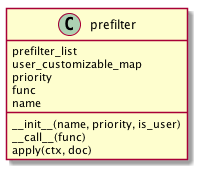
\includegraphics[width=0.4\textwidth]{img/prefilter.png}
    \caption{Prefilter\label{fig:prefilter}}
  \end{figure}

  \subsubsection{Function}
    Prefilter is the first classifier applied on the information. It can be system defined or user customized.
    Itself has priority levels, thus different prefilter will be executed on a information in order.
    It will put different tags on a piece of information, so in the next step it can be selected out easily.

  \subsubsection{Performance}
    It shall give the result almost immediately after it was called. So it only has several seconds of time.

  \subsubsection{Input}
    A FetcherContext item which was just fetched by a fetcher.

  \subsubsection{Output}
    A FetcherContext item which has multiple tags base on its content read by prefilter.
    Notice that a item may be abandoned by a prefilter for it may be duplicate, redundant or illegal.

